\section{Histogram \cite{data/online/seaborn.histplot}} \label{Visualizing Data/Histogram}


\begin{table}[H]
\begin{minipage}[t]{0.35\linewidth}
\begin{figure}[H]
    \centering
    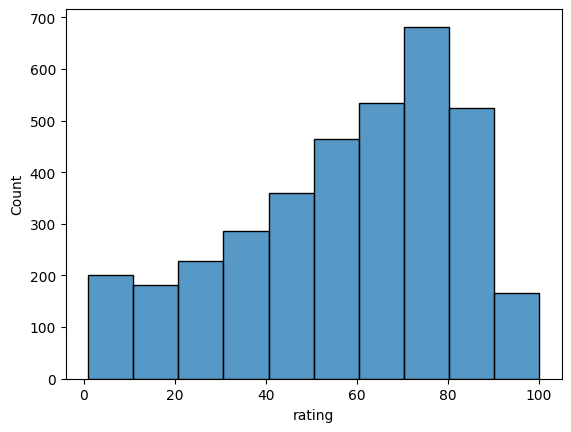
\includegraphics[width=0.9\linewidth, height=10cm, keepaspectratio]{images/data/__visualizations__/sns-hist-rating-face-data.png}
    \caption{Histogram (py-sns) output (face\_data.csv)}
\end{figure}
\end{minipage}
\hspace{0.2cm}
\vrule width 1pt
\hspace{0.5cm}
\begin{minipage}[t]{0.57\linewidth}
\begin{lstlisting}[
    language=Python,
    caption=Histogram: py-sns: face\_data.csv
]
sns.histplot(df["rating"], binwidth=10)
plt.show()
\end{lstlisting}

\vspace{0.2cm}

\begin{enumerate}
    \item A histogram is a classic visualization tool that represents the distribution of one or more variables by counting the number of observations that fall within discrete bins. \hfill \cite{data/online/seaborn.histplot}

    \item A histogram “bins” the data (discretizes it), and subsequently shows the frequency of occurrence in each bin. \hfill \cite{statistics/book/Statistics-for-Data-Scientists/Maurits-Kaptein}

    \item It is the continuous variant of the bar chart. \hfill \cite{statistics/book/Statistics-for-Data-Scientists/Maurits-Kaptein}\\
    SEE: \fullref{Visualizing Data/Box and Whiskers Plot or Box Plot}

    \item The number of bins selected makes a big difference in the visualization: too few bins obscure the patterns in the data, but too many bins lead to counts of exactly one for each value. \hfill \cite{statistics/book/Statistics-for-Data-Scientists/Maurits-Kaptein}
\end{enumerate}

\end{minipage}
\end{table}
